%\documentclass[iop]{emulateapj}
%\documentclass[12pt, preprint]{emulateapj}
\documentclass[12pt, onecolumn]{emulateapj}

\usepackage{amsmath}
%\usepackage{bibtex}
%\bibliographystyle{unsrtnat}

\usepackage{tikz}
\usetikzlibrary{shapes.geometric, arrows}
\usetikzlibrary{fit}
\usetikzlibrary{arrows.meta}

\tikzstyle{hyper} = [circle, text centered, draw=black]%, fill=blue!30]
\tikzstyle{param} = [circle, text centered, draw=black]%, fill=green!30]
\tikzstyle{data} = [circle, text centered, draw=black, line width=2pt]%, fill=red!30]
%\tikzstyle{hyper} = [trapezium, trapezium left angle=70, trapezium right angle=110, minimum width=1cm, minimum height=0.5cm, text centered, draw=black, fill=green!30]
%\tikzstyle{param} = [rectangle, minimum width=1cm, minimum height=0.5cm, text centered, draw=black, fill=green!30]
%\tikzstyle{data} = [diamond, minimum width=1cm, minimum height=1cm, text centered, draw=black, fill=red!30]
%\tikzstyle{eqn} = [rectangle, minimum width=1cm, minimum height=0.5cm, text centered, draw=black]%, fill=green!30]
%\tikzstyle{latent} = [diamond, minimum width=1cm, minimum height=0.5cm, text centered, draw=black]%, fill=green!30]
\tikzstyle{arrow} = [thick,->,>=stealth]
\tikzset{det/.style={insert path={ node {.} }}}

\newcommand{\myemail}{aimalz@nyu.edu}
\newcommand{\textul}{\underline}

%\slugcomment{}

\shorttitle{Probabilistic Redshifts}
\shortauthors{Malz}

\begin{document}

\begin{align}
\end{align}

\title{Redshift Estimation: Avenues for Improvement}

\author{A.I. Malz\altaffilmark{1}}
\altaffiltext{1}{CCPP}
\email{aimalz@nyu.edu}

\begin{abstract}
This document presents a brief introduction to redshift estimation methods for a non-astronomer audience before outlining some open problems in the subject and a brief discussion of possible solutions.
\end{abstract}

\keywords{photo-z}

\section{Introduction}
\label{sec:intro}

Redshift is a measure of the relative velocity between an object and its observer.  It is of scientific relevance to obtain redshifts for galaxies in the universe, in part because the redshift $z$ is proportional to the distance $d$ by Hubble's Law.  Since light travels at a finite speed, more distant galaxies appear as they did at a distant time in the past, enabling study of galaxy evolution. 

The redshift may be observed by taking a spectrum, a measurement of the energy flux $f(\lambda)$ carried by photons from a galaxy over a range of wavelengths $\lambda$, and determining the displacement of recognizable features, such as atomic or molecular emission or absorption lines.  However, spectra are only available for the brightest galaxies, making them impractical for the study of distant galaxies.  The "poor man's" spectrum is photometry, an extremely coarse spectrum comprised of flux transmitted through each of several filters $q$ of transmittance $r_{q}(\lambda)$.

Given $Q$ filter throughputs $f_{q}$, an estimate of the initial spectrum $f(\lambda)$ is made.  This coarse spectrum is fit to a redshift either by assuming a library of physically motivated redshifted template spectra or by deriving an effective basis of spectral templates from a training set with spectroscopically confirmed redshifts.  Typically, the redshift we wish to estimate $\hat{z}$ is reported as the redshift $z^{t}$ of the best fit (as measured by $\chi^{2}$) template spectrum with some Gaussian error $\sigma^{2}$ based on the goodness of that fit and observational uncertainties on $f_{q}$.

Rather than making point estimates, it would be advantageous to estimate probability distribution functions (zPDFs) on redshifts of individual galaxies.  There are several interesting questions one may ask about such a procedure.  Before discussing these questions, let us establish some notation and review some background relevant to probability.

Let's say we have some data $\vec{d}_{n}$ from a galaxy $n$ in a survey of $N$ galaxies.  Though additional information may be included in $\vec{d}_{n}$, at the very least it must contain the $f_{n}^{n}$ that comprise the photometry.  Instead of being given energy fluxes $f_{q}^{n}$, sometimes magnitudes $m_{q}^{n}\propto -\log f_{q}^{n}$ are provided.  In some cases, we are instead given $Q-1$ "colors" $c_{q}^{n}=m_{q+1}^{n}-m_{q}^{n}$ with one magnitude $m_{0}$ that may be used to calculate the original $\vec{m}_{n}$ from which the colors were derived.  We would like to use this data to estimate the parameter $z_{n}$ representing the galaxy's redshift.  

Point estimates $\hat{z}_{n}$ suffer from various weaknesses that affect the science we can do with them that are best illustrated by comparing $\hat{z}_{n}$ versus $z_{n}$ for a set of test data with known redshifts.  Since both template fitting and machine learning methods essentially match photometry to a template or basis spectrum with both an intrinsic spectrum and a redshift, there are errors associated with misassignment of both redshift and intrinsic spectra to $\vec{d}_{n}$.  Catastrophic errors occur when $|z_{n}-\hat{z}_{n}|$ is quite large, although another insidious type of error occurs when many galaxies near some $z$ sharing some feature are assigned redshift estimates near some $\hat{z}$ elsewhere. 

Instead, we would like to work with a redshift probability distribution function for each galaxy.  We recall Bayes' Theorem, the relationship between the likelihood $p(\vec{d}_{n}|z)$ (the probability of observing the data at each value of the continuous parameter $z$) and the posterior $p(z|\vec{d}_{n})$ (the probability of each value of the continuous parameter $z$ given the observed data): $p(\vec{d}_{n}|z)p(z)=p(z|\vec{d}_{n})p(\vec{d}_{n})$.  Because any estimate of redshift by template fitting or machine learning will implicitly have to be marginalized over some nuisance parameters $\{\vec{t}_{j}\}_{J}$ representing the estimator of the intrinsic spectrum (also known as the spectral energy distribution or SED), it is considered much easier to find the posterior $p(z|\vec{d}_{n})=\int\ p(z,\vec{t}|\vec{d}_{n})\ p(\vec{t})\ d\vec{t}$, which we shall refer to as zPDF from this point forward.

\subsection{Open Questions}

Here are some interesting questions we may ask about zPDFs:

\begin{enumerate}
%\item \label{it:likelihood} How can redshift likelihood functions, as opposed to posterior probability distributions, be estimated?
\item \label{it:posterior} What methods are appropriate and effective for generating posterior zPDFs from photometric data?
\item \label{it:single} How can one estimate a zPDF from a single band of photometry?
\item \label{it:plus} How much is an estimate of a zPDF improved by the inclusion of each additional band of photometry? 
\item \label{it:pixel} How can one use photometry at each pixel in a galaxy to generate a posterior zPDF?
\item \label{it:spatial} How informative is inclusion of the angular size of a galaxy to the estimated zPDF?
\item \label{it:croscor} How may position information be used to improve zPDFs?
\item \label{it:inference} How should zPDFs be used in inference?
\end{enumerate}

These questions will each be discussed in detail below.

\section{Generation of zPDFs}

Question \ref{it:posterior} pertains to the processing of data $\vec{d}_{n}$ to estimate the distribution of parameters $p(z|\vec{d}_{n})$.  Previous work on obtaining zPDFs has employed similar methods to those used to obtain point estimates. Data-driven $k$-nearest neighbor algorithms have been implemented by \citet{she11} neglecting measurement errors and by \citet{bal08} including measurement errors.  \citet{bon13} uses neural-networks to obtain zPDFs.  \citet{car13} use prediction tree and random-forest classification techniques and \citet{car14} use self-organizing maps  to obtain zPDFs.  An extension of \citet{ben00} that produces full posteriors (as opposed to a selection of local maxima) from a template library has been mentioned in the litertature (see \citet{lop14}), but a formal presentation has not yet been published.

Any progress in answering Question \ref{it:posterior} would be extremely relevant to the upcoming Large Synaptic Survey Telescope (LSST), which will produce high-quality photometry on 20 billion objects down to an unprecedented brightness limit.  The collaboration has stated the intention of producing zPDFs and has included some investigation of the feasibility of this goal, including use of techniques relevant to Question \ref{it:croscor}, in Sec. 3.8 of \citet{abe09}.

No existing method producing zPDFs has provided an explicit statement of the prior distribution $p(\vec{t})$ (parametrized by $\vec{T}$) of nuisance parameters $\{\vec{t}_{j}\}_{J}$ employed in the calculation of zPDFs given in Eq. \ref{eq:prior}, which is essential for using zPDFs for inference.  In doing inference, we value a notion of "trust" of the zPDFs we use; a trustworthy posterior zPDF must be calculated from a trustworthy prior, and a trustworthy prior must be derived from a complate (or completeable) training set (whether data-driven or template-based) spanning the space of photometry $\{\vec{d}_{n}\}_{N}$, redshifts $\{z_{n}\}_{N}$, and nuisance parameters $\{\vec{t}_{n}\}_{N}$ for the test set of data for which we would like to obtain posteriors $p(z|\vec{d}_{n})$.  

\begin{align}
\label{eq:prior}
p(z|\vec{d}_{n}) &= \int p(z,\vec{t}|\vec{d}_{n})p(\vec{t})d\vec{t}
\end{align}

It would be interesting to consider a variety of choices for the hyperparameters $\vec{T}$, including those that do not effectively span the space of data and parameters, and determine their effects on inference of hyperparameters $\vec{\theta}$ in $p(\vec{\theta}|\{\vec{d}_{n}\}_{N})$.  Some work along these lines has been done for the upcoming LSST survey, namely an investigation of the effect on point estimates of photometric redshift due to use of a limited set of template/training set spectra $\{\vec{t}_{j}\}_{J}$.  \citep{abe09}

A related idea (related to the answer to Question \ref{it:croscor} in the absence of positional information) is to cross-correlate the locations of training and test set galaxies in color and redshift-space.  This could involve choosing a prior related to a summary statistic such as a number density of galaxies over redshift and color.  This approach seems to be a simple extension of the work of \citet{she11}.

\subsection{Single-band photometry}

Question \ref{it:single} is about the special case in which $\vec{d}_{n}=m_{n}$, a scalar representing the magnitude in one photometric filter.  If we were to calculate $p(z_{n}|m_{n})$ from such limited data, could it be used for meaningful inference?  I suspect $m_{n}$ would be a very noisy proxy for distance, since the flux is proportional to the inverse square of the distance to the source and a single pixel carries no spectral information.  Noise would be introduced by the very characteristics in galaxy spectra that permit point estimates of redshift to be made.

\subsection{Marginals of multi-band photometry}

Question \ref{it:plus} is easy to answer given the answer to question \ref{it:single}.  In other words, how would the estimate of $p(z_{n}|\vec{d}_{n})$ change if the length of $\vec{m}_{n}$ were $Q+1$ instead of $Q$?  This could be done by repeating whatever procedure was done to answer question \ref{it:single} with the addition of another filter.  One can ask what the minimum $Q$ is that makes the posterior $p(z_{n}|\{m_{n}\}_{Q})$ sufficiently precise for a particular science goal.  This work could help future surveys get the maximum "bang for their buck" by optimizing the choice of number and spectral range of filters.

\subsection{Spatial information to refine zPDFs}

Question \ref{it:pixel} makes use of pixel-level data to incorporate discrepancies in photometry across the extent of a galaxy in the focal plane into the zPDF.  An answer to this question makes some assumptions about the cause for multimodal zPDFs, namely that the photometry $\vec{m}_{n}$ in those cases varies across pixels $l=1,\dots,L$.  If multimodal zPDFs are a result of the width of the filters imposing an inherent degeneracy in the training set's color space with respect to the nuisance parameters $\{\vec{t}_{n'}\}_{N'}$ and redshifts $\{z_{n'}\}_{N'}$ then this assumption is untrue and pixel-level photometry would not improve zPDFs.

\subsection{zPDFs derived from a prior including imaging information}

Question \ref{it:spatial} is about possible use of angular size, surface brightness, or morphological information to refine zPDFs, rather than simply using a prior on photometric magnitudes as was first done in \citet{ben00}.  \citet{vak15} is investigating the improvement in data-driven redshift point estimates resulting from inclusion of angular size in $\{\vec{d}_{n}\}_{N}$ and $\{\vec{d}_{n'}\}_{N'}$.  \citet{sta07} discusses a prior on surface brightness in making redshift point estimates.  It is possible that such methods could be extended to generation of zPDFs.

\subsection{Cross-correlation zPDFs}

Question \ref{it:croscor} stems from the observed correlation of redshifts between galaxies near one another on the sky, caused by the fact that many galaxies are gravitationally bound to their neighbors in physical space.  For this discussion, let us say we have $M$ pairs of galaxies $(n,n')$ near one another with test set data $\textul{d}_{n}$ comprised of photometry $\vec{m}_{n}$ and position $\vec{\phi}_{n}$ as well as training set data $\textul{d}_{n'}$ comprised of photometry $\vec{m}_{n'}$, position $\vec{\phi}_{n'}$, and a reliable redshift $z_{n'}$.  

There are two current techniques in place for determining $z_{n}$.  The first is to set $\hat{z}_{n}=z_{n'}$ for all galaxies with $\Delta_{nn'}=|\vec{\phi}_{n'}-\vec{\phi}_{n}|$.  The second is to draw $\hat{z}_{n}$ from a normal distribution centered at $z_{n'}$ with a variance $\sigma^{2}_{n'}$ derived from some combination of $\Delta_{nn'}$ and $z_{n'}$.  One possible approach to improving this method would be to work with the actual posterior distribution $p(z_{n}|\textul{d}_{n})\sim N(z_{n'},\sigma^{2}_{n'})$ rather than samples, although that could be prohibitively computationally expensive.

Another solution takes advantage of our knowledge of the angular and/or redshift-space and/or real-space correlation functions $\vec{\xi}$ for galaxies.  This approach has been indirectly suggested by \citet{sch06} for point estimates of redshift, which was applied by \citet{rah14} to SDSS galaxies. Since $\vec{\xi}$ is defined at all angular separations, such a method could be used to improve zPDFs not just of neighboring galaxies but of every galaxy in a survey.  

One proposal for how to get around the issue of untrustworthy priors mentioned in response to Question \ref{it:posterior} is so-called cross-correlation redshifts that take advantage of the fact that the relationship between the angular cross-correlation function $\vec{\xi}_{sp}$ of training set galaxies at $\vec{\phi}^{s}_{n'}$ and test set galaxies at $\vec{\phi}^{p}_{n}$ can be used as a prior on the estimation of other parameters describing the redshift distribution, such as the redshift density function $n(z)$ \citep{new08}, \citep{men13} and redshift distribution function $N(z)$ \citep{mat10}.  However, cross-correlation redshifts are a natural extension to the approach of simultaneous inference of zPDFs and $\vec{\xi}$ proposed in response to Question \ref{it:inference}.

Given the redshift density function $n_{p}(z)$ for a test set and If we wish to estimate the comoving number density of test set galaxies $n_{p}(r,z)$ as a function of the redshifts and comoving physical distances $r(z)$ from each training set galaxy to each test set galaxy given an observed angular cross-correlation $\xi_{sp}(r,z)$ between the comoving physical distances and redshifts of test and training set galaxies ,  \citep{new08}

This method has not yet been adapted to handle individual redshift posteriors for the test set and permits neither refinement of the input photometric redshifts nor determination of individual redshift posteriors based on $n(z)$ and $\vec{\xi}_{sp}$.  It is worth reviewing the method in detail to investigate possible extensions to zPDFs.

\section{Toy Problem: Sample Discrimination}

Consider a survey in which all galaxies have one of exactly two redshifts sufficiently apart that one would expect no correlation between the power spectra at each redshift.  In the case in which we are interested solely in one group and not in the other, hereafter referred to as the contaminating population, we wish to estimate the power spectrum of that group given some incompleteness and contamination.  In this case, the three dimensional galaxy map is a linear combination of galaxies from each of the two populations, and since the two possible redshifts are distant from one another, the power spectrum of the combined sample will be a linear combination of the power spectra of each individual population.  In this problem, several questions can be investigated.

\begin{itemize}
\item Can we analytically solve for the power spectrum of the population of interest in terms of the observed power spectrum and contamination/incompleteness fractions?
\item Can the observed power spectrum of the two groups be used to identify misclassified galaxies and reclassify their redshifts in an iterative calculation of the power spectrum?
\item If instead of deterministic redshift assignments we have probabilities for each galaxy, can they be used to infer the posterior of the power spectrum of interest?
\end{itemize}

This problem is also similar to that of blended objects, in which we observe more than one galaxy but classify it as a single galaxy due to the close proximity on the sky of the galaxies in question.  Redshift estimation in this case can be catastrophically wrong, but discrimination of blended systems could be valuable in improving the power spectrum calculated from the blended galaxy map.  Again, in this toy model, it would be of interest to investigate how the observed power spectrum is affected by blended objects and whether it can be corrected through an iterative procedure on the identification of blended systems.

\section{zPDFs in inference}

zPDFs have been used in the literature to estimate parameters relevant to cosmology and galaxy evolution, including the redshift density function (\citet{she11}, \citet{bon13}, and \citet{vii15}), angular cross-correlation function \citep{mye09}, and merger fraction \citep{lop14}.  However, not all published applications are mathematically consistent.   Question \ref{it:inference} is currently being investigated by \citet{mal15}, with a focus on one-point statistics of redshift such as the redshift distribution function $N(z)$, the redshift density function $n(z)$, and the weak lensing mean distance ratio.

Future work is planned for use of zPDFs in higher-order statistics for cosmology, such as angular correlation functions and weak gravitational lensing shear fields, as has been done by \citet{man07}.  (It is likely that direct application of any theoretical results of such an investigation would be computationally prohibitive, so MCMC methods would probably need to be employed to advance estimators of such statistics.)  These statistics have the added complication of observables other than $\{\vec{m}_{n}\}_{N}$, including angular positions $\vec{\phi}=(\alpha,\delta)$.  

One avenue to explore is to combine Questions \ref{it:posterior} and \ref{it:inference} to simultaneously determine both the posteriors of the individual galaxies $p(z|\vec{d}_{n})$ and the hyperparameters of interest $p(\vec{\theta}|\{\vec{d}_{n}\}_{N})$.  A first stab at this possibility is demonstrated by the hierarchical model displayed graphically by Fig. \textbf{redacted}, applicable to the angular correlation function.  (For the weak lensing shear field, there would be additional parameters for the shape $\vec{S}_{n}$ that would have to be implicitly estimated along with the posteriors over redshift like the SEDs $\vec{t}_{n}$ in Eq. \ref{eq:prior}.)  An equation summarizing the generative model presented in Fig \textbf{redacted} is given by Eq. \textbf{redacted}.

%\begin{figure}
%\label{fig:inference}
%\vspace{0.5cm}
%\begin{center}
%\begin{tikzpicture}[node distance=1cm]
%
%\node (powspec) [hyper] {$\vec{\mathcal{P}}$};
%\node (nz) [hyper, below of=powspec, xshift=+0.75cm] {$\vec{\mathcal{N}}$};
%\node (croscor) [hyper, below of=powspec, xshift=-0.75cm] {$\vec{\xi}$};
%\node (prior) [hyper, below of=powspec,xshift=+2cm] {$\vec{T}$};
%\node (z) [param, below of=nz, yshift=-0.25cm] {$z_{n}$};
%\node (nuisance) [param, below of=prior, yshift=-0.25cm] {$\vec{t}_{n}$};
%\node (ang) [data, below of=croscor, yshift=-0.5cm] {$\Delta_{n,n'}$};
%\node (anglab) [yshift=-0.25cm] at (ang.south) {$n'=1,\dots,N'$};
%\node (mags) [data, below of=z,yshift=-0.25cm,xshift=+0.5cm] {$\vec{m}_{n}$};
%%\node (pos) [data, below of=ang,yshift=-0.25cm] {$\vec{\phi}_{n}$};
%\node (survey) [draw=black,fit={(nuisance.east)(ang.north)(mags.south)(anglab.west)}] {};
%\node (survlab) [xshift=+2.5cm,yshift=-0.25cm] at (survey.south) {$n=1,\dots,N$};
%
%\draw [arrow] (prior) -- (nuisance);
%\draw [arrow] (powspec) -- (nz);
%\draw [arrow] (powspec) -- (croscor);
%\draw [arrow] (nz) -- (z);
%\draw [arrow] (z) -- (mags);
%\draw [arrow] (nuisance) -- (mags);
%\draw [arrow] (croscor) -- (ang);
%%\draw [arrow] (ang) -- (pos);
%
%\end{tikzpicture}
%\caption{This directed acyclic graph illustrates a generative model in which the hyperparameters $\vec{\mathcal{P}}$ determining the power spectrum may be projected into the angular correlation function parametrized by $\vec{\xi}$ and redshift distribution function parametrized by $\vec{\mathcal{N}}$.  Thus $\vec{\mathcal{P}}$ is effectively separable into components contributing to observable angular distances $\{\Delta_{nn'}\}_{N'}$ and redshifts $z_{n}$ we will have to estimate from the observable brightness $\vec{m}_{n}$ that may be considered independently.  (Though the position $\vec{\phi}_{n}$ is truly what is observed, we may assume that $\{\Delta_{nn'}\}_{N'}$ is a simple transformation of perfectly measured $\vec{\phi}_{n}$ and $\{\vec{\phi}_{n'}\}_{N'}$.)  The effect of the nuisance parameters $\vec{t}_{n}$ cannot be disentangled from that of $z_{n}$ in determining $\vec{m}_{n}$, but they are constraied by the parameters $\vec{T}$ which may have a strong prior.}
%\end{center}
%\end{figure}

%\begin{align}
%\label{eq:fullcc}
%p(\mathcal{P}|\{(\{\Delta_{nn'}\}_{N'},\vec{m}_{n})\}_{N}) =& \ p(\vec{P})\prod_{n=1}^{N}\iint\left[\iint p(\vec{t}_{n}|\vec{T})\ p(z_{n}|\vec{\mathcal{N}})\ p(\{\Delta_{nn'}\}_{N'}|\vec{\xi})\ p(\vec{T})\ p(\vec{\mathcal{N}},\vec{\xi}|\vec{\mathcal{P}})\ d\vec{T}\ d\vec{\mathcal{N}}\ d\vec{\xi}\right]\\
%& %\ \ \ \ \ \ \ \ \ \ 
%\indent\indent\indent\indent\indent\indent\indent p(\vec{m}_{n}|\vec{t}_{n},z_{n})\ d\vec{t}_{n}\ dz_{n}\ d\{\Delta_{nn'}\}_{N'}
%\end{align}

\dots

\subsection{One-point statistics}

\subsubsection{One-point statistic of redshift}

The simplest one-point statistic of redshift is the redshift distribution function.  The probabilistic graphical model of Malz \& Hogg 2016 is given in Fig. \ref{fig:nz}. 

\begin{figure}
\vspace{0.5cm}
\begin{center}
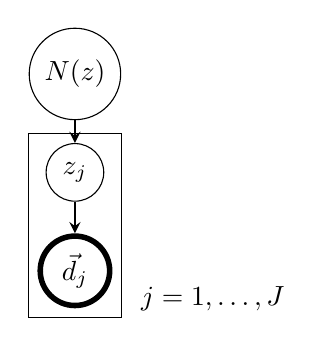
\begin{tikzpicture}[node distance=1cm]

\node (nz) [hyper] {$N(z)$};
\node (z) [param, below of=nz,yshift=-0.25cm] {$z_{j}$};
\node (mags) [data, below of=z,yshift=-0.25cm] {$\vec{d}_{j}$};
\node (survey) [draw=black,fit={(mags.west)(z.north)(mags.south)(mags.east)}] {};
\node [xshift=1.75cm,yshift=0.25cm] at (survey.south) {$j=1,\dots,J$};

\draw [arrow] (nz) -- (z);
\draw [arrow] (z) -- (mags);

\end{tikzpicture}
\caption{}
\label{fig:nz}
\end{center}
\end{figure}

In general, redshift is degenerate with nuisance parameters, namely the galaxy SED $\vec{\alpha}$.

\begin{figure}
\vspace{0.5cm}
\begin{center}
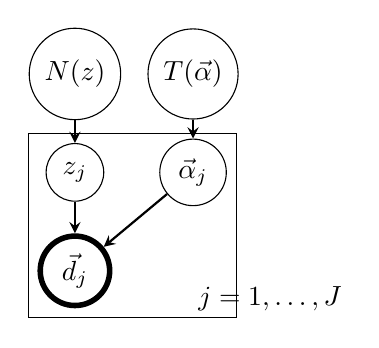
\begin{tikzpicture}[node distance=1cm]

\node (nz) [hyper] {$N(z)$};
\node (talpha) [hyper,xshift=1.5cm] {$T(\vec{\alpha})$};
\node (z) [param, below of=nz,yshift=-0.25cm] {$z_{j}$};
\node (sed) [param, below of=talpha,yshift=-0.25cm] {$\vec{\alpha}_{j}$};
\node (mags) [data, below of=z,yshift=-0.25cm] {$\vec{d}_{j}$};
\node (survey) [draw=black,fit={(mags.west)(z.north)(mags.south)(sed.east)}] {};
\node [xshift=1.75cm,yshift=0.25cm] at (survey.south) {$j=1,\dots,J$};

\draw [arrow] (nz) -- (z);
\draw [arrow] (talpha) -- (sed);
\draw [arrow] (sed) -- (mags);
\draw [arrow] (z) -- (mags);

\end{tikzpicture}
\caption{}
\label{fig:nuisance}
\end{center}
\end{figure}

\subsubsection{One-point statistic of redshift and a scalar parameter}

We consider a second parameter $M_{j}$ that may represent the luminosity or mass of a galaxy $j$ in a survey.  We assume we are given a survey of joint posteriors $\{p(z_{j},M_{j}|\vec{d}_{j})\}_{J}$.  Fig. \ref{fig:mf} illustrates the conditionals of such a problem.  (ALHAMBRA, for example, produces posteriors of this form with a binning parametrization.)

\begin{figure}
\vspace{0.5cm}
\begin{center}
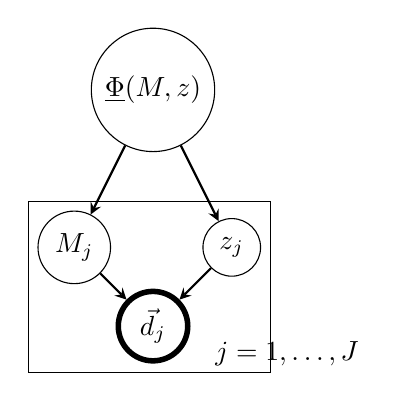
\begin{tikzpicture}[node distance=1cm]

\node (mf) [hyper,xshift=-1cm] {$\textul{\Phi}(M,z)$};
%\node (nz) [hyper,xshift=0.5cm,yshift=-1cm] {$N(z)$};
\node (z) [param, below of=mf,yshift=-1cm,xshift=1cm] {$z_{j}$};
\node (M) [param, below of=mf,yshift=-1cm,xshift=-1cm] {$M_{j}$};
\node (flux) [data, below of=mf,yshift=-2cm] {$\vec{d}_{j}$};
\node (survey) [draw=black,fit={(M.west)(M.north)(flux.south)(z.east)}] {};
\node [xshift=1.75cm,yshift=0.25cm] at (survey.south) {$j=1,\dots,J$};

\draw [arrow] (mf) -- (z);
\draw [arrow] (mf) -- (M);
\draw [arrow] (z) -- (flux);
\draw [arrow] (M) -- (flux);

\end{tikzpicture}
\caption{}
\label{fig:mf}
\end{center}
\end{figure}

\begin{align*}
p(\textul{\Phi}|\{\vec{d}_{j}\}_{J}) &= \frac{p(\textul{\Phi})}{p(\{\vec{d}_{j}\}_{J})}p(\{d_{j}\}_{J}|\textul{\Phi})\\
&\propto p(\textul{\Phi})\prod_{j=1}^{J}p(\vec{d}_{j}|\textul{\Phi})\\
&\propto p(\textul{\Phi})\prod_{j=1}^{J}\iint p(\vec{d}_{j}|z_{j},M_{j})p(z_{j},M_{j}|\textul{\Phi})dz_{j}dM_{j}\\
&\propto p(\textul{\Phi})\prod_{j=1}^{J}\iint p(\vec{d}_{j}|z_{j},M_{j})\frac{p(M_{j},z_{j}|\vec{d}_{j},\textul{\Phi}_{0})}{p(M_{j},z_{j}|\vec{d}_{j},\textul{\Phi}_{0})}p(z_{j},M_{j}|\textul{\Phi})dz_{j}dM_{j}\\
&\propto p(\textul{\Phi})\prod_{j=1}^{J}\iint p(\vec{d}_{j}|z_{j},M_{j})p(M_{j},z_{j}|\vec{d}_{j},\textul{\Phi}_{0})\frac{p(\vec{d}_{j}|\textul{\Phi}_{0})}{p(\vec{d}_{j}|z_{j},M_{j},\textul{\Phi}_{0})p(z_{j},M_{j}|\textul{\Phi}_{0})}p(z_{j},M_{j}|\textul{\Phi})dz_{j}dM_{j}\\
&\propto p(\textul{\Phi})\prod_{j=1}^{J}\iint \frac{p(M_{j},z_{j}|\vec{d}_{j},\textul{\Phi}_{0})}{p(z_{j},M_{j}|\textul{\Phi}_{0})}\frac{p(\vec{d}_{j}|z_{j},M_{j})p(\vec{d}_{j}|\textul{\Phi}_{0})}{p(\vec{d}_{j}|z_{j},M_{j},\textul{\Phi}_{0})}p(z_{j},M_{j}|\textul{\Phi})dz_{j}dM_{j}\\
&\propto p(\textul{\Phi})\prod_{j=1}^{J}\iint \frac{p(M_{j},z_{j}|\vec{d}_{j},\textul{\Phi}_{0})}{p(z_{j},M_{j}|\textul{\Phi}_{0})}p(z_{j},M_{j}|\textul{\Phi})dz_{j}dM_{j}\\
&\propto p(\textul{\Phi})\prod_{j=1}^{J}\iint p(M_{j},z_{j}|\vec{d}_{j},\textul{\Phi}_{0})\frac{p(z_{j},M_{j}|\textul{\Phi})}{p(z_{j},M_{j}|\textul{\Phi}_{0})}dz_{j}dM_{j}
\end{align*}

\subsubsection{One-point statistic of redshift and a vector of parameters}

Let us consider the three-dimensional lensing potential $\textul{\psi}$ estimated from a survey of $N$ galaxy fluxes $\{\vec{f}_{n}\}_{N}$ and angular positions $\{\vec{\theta}_{n}\}_{N}$.  We assume the following quantities are known: $\{p(z_{n}|\vec{f}_{n})\}_{N}$, $\{p(z_{n}|\vec{x}_{n})\}_{N}$, $\{p(\vec{x}_{n}|\textul{\psi})\}_{N}$, $p(\vec{x}_{n}|\vec{\theta}_{n},z_{n}\}_{N}$.  We will have to employ interim priors $\textul{\psi}_{0}$ and $\{\vec{x}_{n,0}\}_{N}$.

\begin{figure}
\vspace{0.5cm}
\begin{center}
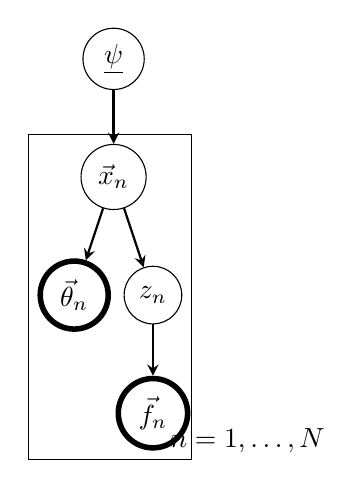
\begin{tikzpicture}[node distance=1cm]

\node (lp) [hyper] {$\textul{\psi}$};
\node (pos) [param, below of=lp,yshift=-0.5cm] {$\vec{x}_{n}$};
\node (z) [param, below of=pos,yshift=-0.5cm,xshift=0.5cm] {$z_{n}$};
\node (t) [data, below of=pos,yshift=-0.5cm,xshift=-0.5cm] {$\vec{\theta}_{n}$};
\node (flux) [data, below of=z,yshift=-0.5cm] {$\vec{f}_{n}$};
\node (survey) [draw=black,fit={(t.west)(pos.north)(flux.south)(z.east)}] {};
\node [xshift=1.75cm,yshift=0.25cm] at (survey.south) {$n=1,\dots,N$};

\draw [arrow] (lp) -- (pos);
\draw [arrow] (pos) -- (z);
\draw [arrow] (pos) -- (t);
\draw [arrow] (z) -- (flux);

\end{tikzpicture}
\caption{}
\label{fig:lenspot}
\end{center}
\end{figure}

\begin{align*}
p(\textul{\psi}|\{\vec{\theta}_{n},\vec{f}_{n}\}_{N}) &= \frac{p(\textul{\psi})}{p(\{\vec{\theta}_{n},\vec{f}_{n}\}_{N})}p(\{\vec{\theta}_{n},\vec{f}_{n}\}_{N}|\textul{\psi})\\
&\propto p(\textul{\psi})p(\{\vec{\theta}_{n},\vec{f}_{n}\}_{N}|\textul{\psi})\\
&\propto p(\textul{\psi})\prod_{n=1}^{N}p(\vec{\theta}_{n},\vec{f}_{n}|\textul{\psi})\\
&\propto p(\textul{\psi})\prod_{n=1}^{N}\int p(\vec{\theta}_{n},\vec{f}_{n}|\vec{x}_{n})p(\vec{x}_{n}|\textul{\psi})d\vec{x}_{n}\\
&\propto p(\textul{\psi})\prod_{n=1}^{N}\int p(\vec{x}_{n}|\textul{\psi})\iint p(\vec{f}_{n}|z_{n})p(\vec{\theta}_{n},z_{n}|\vec{x}_{n})d\vec{\theta}_{n}dz_{n}d\vec{x}_{n}\\
\end{align*}
%
%\begin{figure}
%\vspace{0.5cm}
%\begin{center}
%\begin{tikzpicture}[node distance=1cm]
%
%\node (nz) [hyper,xshift=-2cm] {$N(z)$};
%\node (tf) [hyper,xshift=2cm] {$\theta(\vec{L},v,z)$};
%\node (lf) [hyper] {$\Phi(\vec{L},z)$};
%\node (z) [param, below of=lf,yshift=-0.75cm,xshift=-1cm] {$z_{j}$};
%\node (L) [param, below of=z,yshift=-0.75cm,xshift=1cm] {$\vec{L}_{j}$};
%\node (v) [param, below of=z,yshift=-0.75cm,xshift=2cm] {$v_{j}$};
%\node (flux) [data, below of=L,yshift=-1cm] {$\vec{d}_{j}$};
%\node (survey) [draw=black,fit={(z.west)(z.north)(flux.south)(v.east)}] {};
%\node [xshift=2.25cm,yshift=0.25cm] at (survey.south) {$j=1,\dots,J$};
%
%\draw [arrow] (nz) -- (z);
%\draw [arrow] (lf) -- (L);
%\draw [arrow] (lf) -- (z);
%\draw [arrow] (tf) -- (L);
%\draw [arrow] (tf) -- (v);
%\draw [arrow] (z) -- (L);
%\draw [arrow] (v) -- (flux);
%\draw [arrow] (z) -- (flux);
%\draw [arrow] (L) -- (flux);
%
%\end{tikzpicture}
%\caption{}
%\label{fig:tf}
%\end{center}
%\end{figure}
%
%\begin{figure}
%\vspace{0.5cm}
%\begin{center}
%\begin{tikzpicture}[node distance=1cm]
%
%\node (nz) [hyper,xshift=-1cm] {$N(z)$};
%\node (fj) [hyper,xshift=1cm] {$\theta(\vec{L},\sigma,z)$};
%\node (z) [param, below of=nz,yshift=-0.75cm] {$z_{j}$};
%\node (L) [param, below of=z,yshift=-0.75cm,xshift=1cm] {$\vec{L}_{j}$};
%\node (v) [param, below of=z,yshift=-0.75cm,xshift=2cm] {$\sigma_{j}$};
%\node (flux) [data, below of=z,yshift=-2cm,xshift=0.5cm] {$\vec{d}_{j}$};
%\node (survey) [draw=black,fit={(z.west)(z.north)(flux.south)(v.east)}] {};
%\node [xshift=2.25cm,yshift=0.25cm] at (survey.south) {$j=1,\dots,J$};
%
%\draw [arrow] (nz) -- (z);
%\draw [arrow] (tf) -- (L);
%\draw [arrow] (tf) -- (v);
%\draw [arrow] (z) -- (L);
%\draw [arrow] (z) -- (v);
%\draw [arrow] (v) -- (flux);
%\draw [arrow] (z) -- (flux);
%\draw [arrow] (L) -- (flux);
%
%\end{tikzpicture}
%\caption{}
%\label{fig:fj}
%\end{center}
%\end{figure}

\subsection{Two-point statistics}
\subsubsection{Two-point statistics of redshift}

One relevant issue to the application of the two-point correlation function for shear maps is that the choice of tomographic binning strategy affects the inference of cosmological parameters.  (This section has been discussed with Elizabeth Krause and has received significant input from Michael Schneider.)

\begin{figure}
\vspace{0.5cm}
\begin{center}
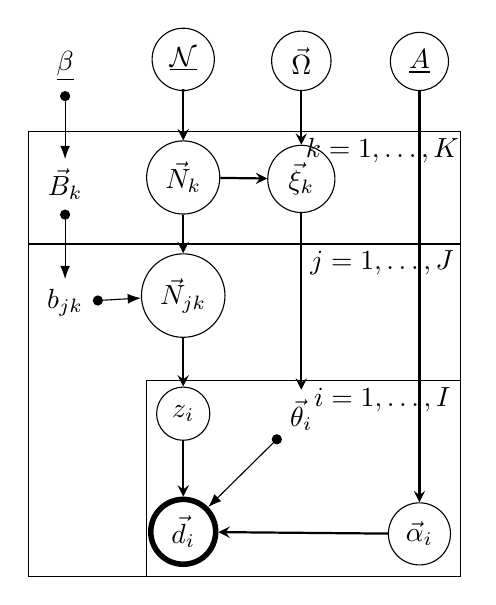
\begin{tikzpicture}[node distance=1cm]

%\node (nz) [det,above] {$\vec{N}$};
\node (n) [hyper,above] {$\textul{\mathcal{N}}$};
\node (nk) [hyper,below of=n,yshift=-0.5cm] {$\vec{N}_{k}$};
\node (nj) [param,below of=nk,yshift=-0.5cm] {$\vec{N}_{jk}$};
\node (zi) [param, below of=nj,yshift=-0.5cm] {$z_{i}$};
\node (di) [data, below of=zi,yshift=-0.5cm] {$\vec{d}_{i}$};

\node (o) [hyper,above,xshift=1.5cm] {$\vec{\Omega}$};
\node (xk) [param,below of=o,yshift=-0.5cm] {$\vec{\xi}_{k}$};
\node (ti) [det, below of=xk,yshift=-2cm] {$\vec{\theta}_{i}$};

\node (b) [det,above,xshift=-1.5cm] {$\textul{\beta}$};
\node (bk) [det,below of=b,yshift=-0.5cm] {$\vec{B}_{k}$};
\node (bj) [det, below of=bk,yshift=-0.5cm] {$b_{jk}$};

\node (a) [hyper,above,xshift=3cm] {$\textul{A}$};
\node (ai) [param, below of=a,yshift=-5cm] {$\vec{\alpha}_{i}$};

\node (g) [draw=black,fit={(zi.west)(ti.north)(di.south)(ai.east)}] {};
\node (s) [draw=black,fit={(bj.west)(nj.north)(di.south)(ai.east)}] {};
\node (c) [draw=black,fit={(bk.west)(nk.north)(di.south)(ai.east)}] {};
\node (gl) [xshift=1cm,yshift=-0.25cm] at (g.north) {$i=1,\dots,I$};
\node (sl) [xshift=1.75cm,yshift=-0.25cm] at (s.north) {$j=1,\dots,J$};
\node (cl) [xshift=1.75cm,yshift=-0.25cm] at (c.north) {$k=1,\dots,K$};

\draw [arrow] (n) -- (nk);
\draw [arrow] (nk) -- (nj);
\draw [arrow] (nk) -- (xk);
\draw [arrow] (nj) -- (zi);
\draw [arrow] (zi) -- (di);

\draw [arrow] (o) -- (xk);
\draw [arrow] (xk) -- (ti);
%\draw [arrow] (ti) -- (di);
\draw[{Circle[black]}-Latex] (ti) -- (di);

%\draw [arrow] (b) -- (bk);
\draw[{Circle[black]}-Latex] (b) -- (bk);
%\draw [arrow] (bk) -- (bj);
\draw[{Circle[black]}-Latex] (bk) -- (bj);
%\draw [arrow] (bj) -- (nj);
\draw[{Circle[black]}-Latex] (bj) -- (nj);

\draw [arrow] (a) -- (ai);
\draw [arrow] (ai) -- (di);

%\draw[{Circle[black]}-Latex] (tj) -- (dj);
%\draw[{Circle[black]}-Latex] (beta) -- (bi);

\end{tikzpicture}
\caption{Here we wish to marginalize over tomographic binning strategies to estimate the cosmological parameters $\vec{\Omega}$.  For each galaxy $i$ in the survey, there is an observed vector of data $\vec{d}_{i}$ determined by the redshift $z_{i}$, the angular position $\vec{\theta}_{i}$, and the intrinsic galaxy properties $\vec{\alpha}_{i}$.  $\textul{\beta}$ contains the parameters determining binning strategies $\vec{B}_{k}$ each with bins $b_{jk}$.  $\textul{\mathcal{N}}$ contains the parameters determining the redshift distribution function with parameters $\vec{N}_{k}$ under each binning strategy, where each bin has a redshift distribution function with parameters in $\vec{N}_{jk}$ that determine the redshifts $z_{i}$.  The cosmological parameters in $\vec{\Omega}$ determine the two-point correlation function parameters $\vec{\xi}_{k}$ which vary over binning strategies $k$, and those determine the angular positions $\vec{\theta}_{i}$.  The intrinsic galaxy parameters $\vec{\alpha}_{i}$ are determined by the hyperparameters contained in $\textul{A}$.}
\label{fig:tomo}
\end{center}
\end{figure}

%\begin{figure}
%\vspace{0.5cm}
%\begin{center}
%\begin{tikzpicture}[node distance=1cm]
%
%%\node (nz) [det,above] {$\vec{N}$};
%\node (nz) [hyper,above] {$\vec{N}$};
%\node (niz) [hyper,below of=nz,yshift=-0.5cm] {$\vec{N}_{i}$};
%\node (zj) [param, below of=niz,yshift=-0.25cm] {$z_{j}$};
%\node (dj) [data, below of=zj,yshift=-0.75cm] {$\vec{d}_{j}$};
%
%\node (cosmo) [hyper,above,xshift=1.5cm] {$\vec{\Omega}$};
%\node (xii) [param,below of=cosmo,yshift=-0.5cm] {$\vec{\xi}_{i}$};
%\node (wj) [data, below of=zj,xshift=1.5cm,yshift=-0.75cm] {$\vec{w}_{j}$};
%
%\node (bj) [param,below of=xii,xshift=-0.75cm,yshift=-0.25cm] {$b_{j}$};
%\node (tj) [det, below of=bj,yshift=-0.25cm] {$\vec{\theta}_{j}$};
%
%\node (bi) [param,below of=xii,xshift=0.75cm,yshift=-0.25cm] {$\vec{B}_{i}$};
%\node (beta) [det, below of=xii,xshift=1.5cm,yshift=-0.25cm] {$\vec{\beta}$};
%
%\node (survey) [draw=black,fit={(dj.west)(zj.north)(dj.south)(wj.east)}] {};
%\node (tomo) [draw=black,fit={(dj.west)(niz.north)(dj.south)(bi.east)}] {};
%\node [xshift=1.75cm,yshift=0.25cm] at (survey.south) {$j=1,\dots,J$};
%\node [xshift=1.75cm,yshift=0.25cm] at (tomo.south) {$i=1,\dots,I$};
%
%\draw [arrow] (nz) -- (niz);
%\draw [arrow] (niz) -- (zj);
%\draw [arrow] (zj) -- (dj);
%\draw [arrow] (cosmo) -- (xii);
%\draw [arrow] (niz) -- (xii);
%\draw [arrow] (wj) -- (dj);
%\draw [arrow] (xii) -- (bj);
%\draw [arrow] (xii) -- (tj);
%\draw[{Circle[black]}-Latex] (tj) -- (dj);
%\draw [arrow] (bj) -- (zj);
%\draw [arrow] (bi) -- (bj);
%\draw[{Circle[black]}-Latex] (beta) -- (bi);
%
%\end{tikzpicture}
%\caption{}
%\label{fig:tomo}
%\end{center}
%\end{figure}
%\begin{figure}
%\vspace{0.5cm}
%\begin{center}
%\begin{tikzpicture}[node distance=1cm]
%
%\node (fz) [hyper] {$\xi(z,|\vec{r}|)$};
%\node (z) [param, below of=fz,yshift=-0.25cm] {$z_{j}$};
%\node (mags) [data, below of=z,yshift=-0.25cm] {$\vec{d}_{j}$};
%\node (survey) [draw=black,fit={(mags.west)(z.north)(mags.south)(mags.east)}] {};
%\node [xshift=1.75cm,yshift=0.25cm] at (survey.south) {$j=1,\dots,J$};
%
%\draw [arrow] (fz) -- (z);
%\draw [arrow] (z) -- (mags);
%
%\end{tikzpicture}
%\caption{}
%\label{fig:fz}
%\end{center}
%\end{figure}



\subsubsection{Two-point statistics of redshift and a scalar parameter}
\subsubsection{Two-point statistics of redshift and a vector of parameters}
\subsection{Higher-order statistics}

%\acknowledgments

%\appendix

\bibliography{references}

\end{document}